\documentclass[12 pt, a4paper]{Article}

%custom Margin
\usepackage[a4paper, bindingoffset=0.2in, left=1in, right=1in, top=1in, bottom=1in, footskip=0.25in]{geometry}
% General packages
\usepackage[english]{babel}
\pagenumbering{arabic}
\usepackage{color}
\usepackage{lettrine}
\usepackage{setspace}
\usepackage{yfonts}
\usepackage{type1cm}

% Graphics packages
\usepackage{graphicx}
\usepackage{rotating}
\usepackage{subfigure}

% Math packages
\usepackage{array}
\usepackage{amsmath}
\usepackage{amsfonts}
\usepackage{amssymb}
\usepackage{geometry}
\usepackage{xparse}
\usepackage{physics}

% Links packages
\usepackage{hyperref}
\usepackage{url}
\usepackage{xcolor}
\hypersetup{
    colorlinks,
    linkcolor={blue!80!black},
    citecolor={blue!80!black},
    urlcolor={blue!80!black}
}

% Tables packages
\usepackage{adjustbox}
\usepackage{multirow}
\usepackage{hhline}
\usepackage{float}
\usepackage[bottom]{footmisc}
\usepackage{booktabs,caption}
\usepackage[flushleft]{threeparttable}
\usepackage[labelfont=sc]{caption}
\captionsetup[table]{skip=0pt}

% citations
\usepackage[round]{natbib}   % omit 'round' option if you prefer square brackets
%\bibliographystyle{plainnat}
%\bibliographystyle{abbrv}
%\bibliographystyle{acm}
%\bibliographystyle{alpha}
%\bibliographystyle{apalike}
%\bibliographystyle{ieeetr}
%\bibliographystyle{plain}
%\bibliographystyle{siam}
%\bibliographystyle{unsrt}

% figures
%\usepackage{subcaption}

\begin{document}
\title{Problem Set 9\\ ECON 833: Computational Methods for Economists}
\author{Mohammad Jakaria}
\maketitle

%\section{ }
Figure-1 shows the steady-state distribution of saving, labor supply, and consumption for each age based on the S-period overlapping generation model with endogenous labor supply model.\\\

Panel(a) of Fig-1 shows the steady-state distribution of individual savings in an 80-period-lived agent. We can see an inverse-U pattern in the saving function. This implies that the amount of saving of an individual increase with the increase in age up to a certain period of life, then it reaches the peak at the age of 55, and after that, the amount of saving starts declining. 
This makes sense because people generally work more at the early ages of life, and when they get older they want to enjoy more leisure.\\\

Panel(b) shows the steady-state distribution of individual labor supply in an 80-period-lived agent. The figure suggests that an individual's labor supply decreases as he grows older. As we already mentioned that when people become older they want to enjoy the leisure and spend money from their past savings.\\\ 

Panel (c) shows the steady-state distribution of individual consumption in an 80-period-lived agent. We can see that the consumption of an individual increases at an increasing rate as an individual grows older. This finding is consistent with what we have observed from the saving and labor supply distribution of the individual for each age.

%\begin{figure}[!b]
\begin{figure}
\begin{center}
\subfigure[Saving]{
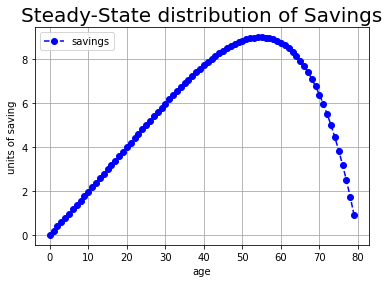
\includegraphics[width=0.60\textwidth]{saving.png}}
\subfigure[Labor Supply]{
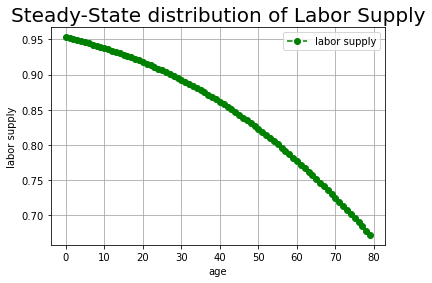
\includegraphics[width=0.60\textwidth]{LaborSupply.png}}
\subfigure[consumption]{
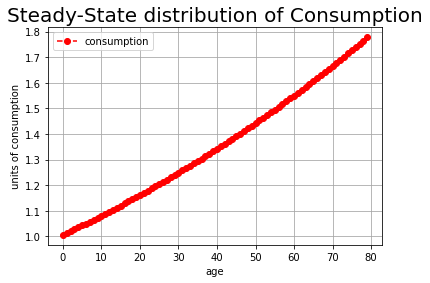
\includegraphics[width=0.60\textwidth]{consumption.png}}
\end{center}
\caption{The steady-state distribution of saving, labor supply, and consumption for each age s}
\end{figure}
%\newpage
%\usepackage{cogsci,pslatex,apacite}
%\usepackage{apacite}
%\bibliographystyle{aea}
%\bibliographystyle{elsarticle-num}
%\bibliographystyle{apacite}
%\bibliography{mybibfile.bib}

\end{document}